\subsection{Gamification module}
\par {The buzz Gamification module is used to manage the game-like presentation of the discussion board by assessing the user contribution, award rewards, and to restrict functionality in the system based on the user level. }
\subsection{Scope}
\par {The scope of the Gamification module is shown in the figure  below}
\begin{figure}[h!]
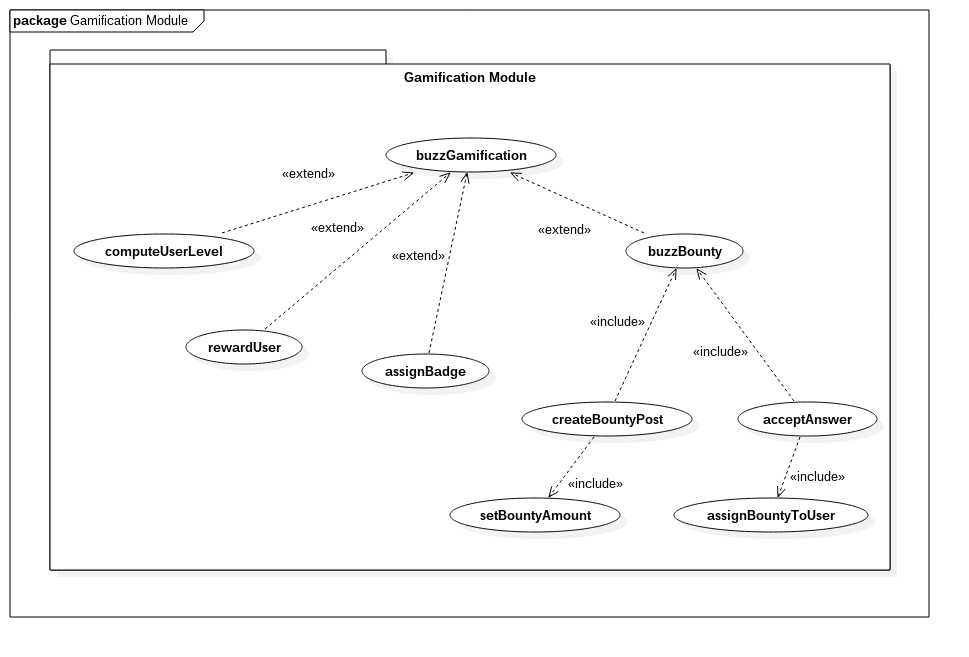
\includegraphics[width=\linewidth]
{Diagrams/Gamification_Scope.jpeg}
\caption {Scope of the Buzz-Gamification module.}
\end{figure}

\subsubsection{Use case}
\par{The use case of the gamification module provide functionality around assessing profiles, awarding rewards, bounty and user level calculation. }

\subsubsection{computeUserLevel}
\par{The system assesses the user profile to calculate the user level in order to restrict the systems functionality and award rewards to a user. The user is assigned a badge according to their level, calculated from the user’s activity, within the system.}

\subsubsection{rewardUser}
\par{The system will allow the user to be rewarded based on their participation within the system, proper use of the system and comments made. A user post receives feedback from posts they make, with the management overseeing the feedback and approval of rewards.}
\subsubsection{Service contracts}
\begin{figure}[h!]
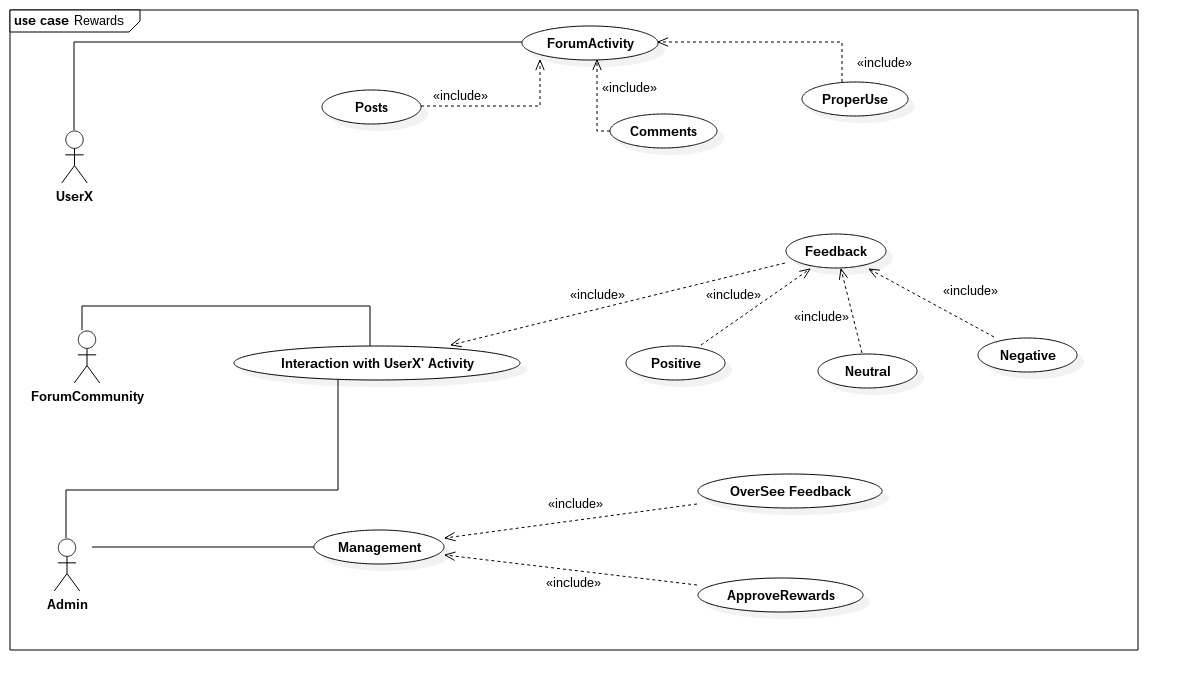
\includegraphics[width=\linewidth]
{Diagrams/rewardUser.jpeg}
\caption {Service contracts of rewardUser.}
\end{figure}

\subsubsection{createBountyPost}
\par{The system will allow the user to create a post and attach a bounty. The bounty functions as points and are given to the user that answers the question correctly. User points can be converted to bounty when creating a post.}

\subsubsection{acceptAnswer}
\par{The system will allow the management of the system oversee and approve an answer to a question posted. Based on his approval, a user may gain or lose their bounty.}

\subsubsection{Domain Model}
\begin{figure}[h!]
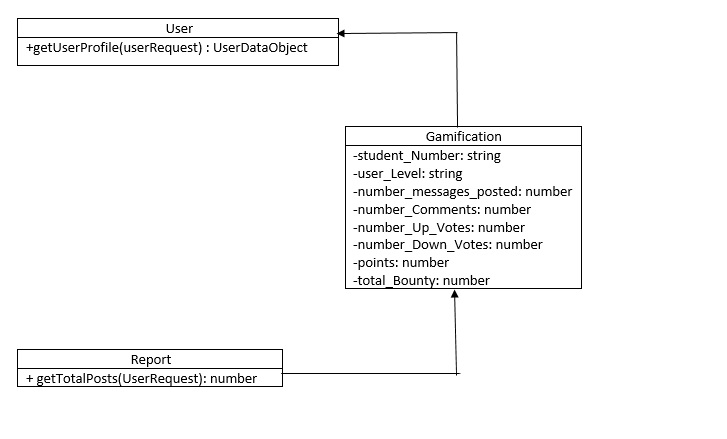
\includegraphics[width=\linewidth]
{Diagrams/gamificationDomainModel.jpeg}
\caption {Domain model of the Buzz-Gamification module.}
\end{figure}
